\subsubsection{UC14 - Gestione ordini - parte vendite}
\begin{figure}[h]
	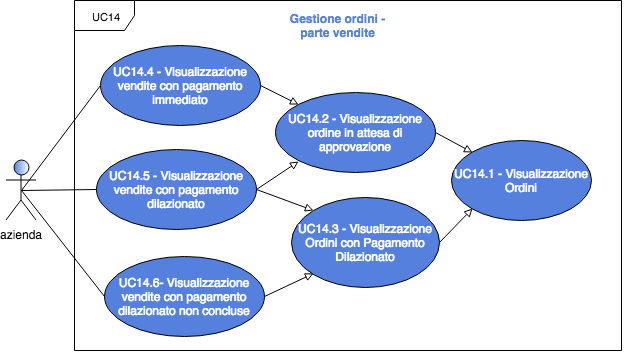
\includegraphics[width=10cm]{res/images/UC14ParteVendite.png}
	\centering
	\caption{Gestione degli ordini dal punto di vista delle vendite}
\end{figure}
\begin{itemize}
	\item \textbf{Attori Primari}: azienda;
	\item \textbf{Descrizione}: alle aziende sono messe a disposizione diverse operazione per visualizzare e gestire le vendite;
	\item \textbf{Scenario principale}: l'utente visualizza e svolge alcune operazioni per gestire le vendite, queste includono:
	\begin{itemize}
		\item visualizzazione della data dell'ordine [UC14.1.1];
		\item visualizzazione del numero dell'ordine [UC14.1.2];
		\item visualizzazione dell'importo netto dell'ordine [UC14.1.3];
		\item visualizzazione dei prodotti inclusi nell'ordine [UC14.1.4];
		\item visualizzazione dell'importo dell'IVA dell'ordine [UC14.1.5];
		\item visualizzazione dell'importo lordo dell'ordine [UC14.1.6].
	\end{itemize}
Inoltre per le vendite in attesa di approvazione è disponibile la data ultima per la conferma [UC14.2.1] e per quanto riguarda gli ordini con pagamento dilazionato,  la data ultima per il pagamento [UC14.3.1].
	\item \textbf{Specializzazione}
	\begin{itemize}
		\item \textbf{UC14.2}: Visualizzazione degli ordini in attesa di approvazione;
		\item \textbf{UC14.3}: Visualizzazione degli ordini con modalità di pagamento dilazionato.
	\end{itemize}
	\item \textbf{Precondizione}: il sistema ha riconosciuto l'utente autenticato come azienda e mette a disposizione tutte le pagine necessarie alla visualizzazione e gestione delle vendite.
	\item \textbf{Postcondizione}: l'azienda ha visualizzato e/o gestito i propri ordini riguardanti le vendite.
\end{itemize} 
\subsubsection{UC14.1 - Visualizzazione Ordini}
\begin{figure}[H]
	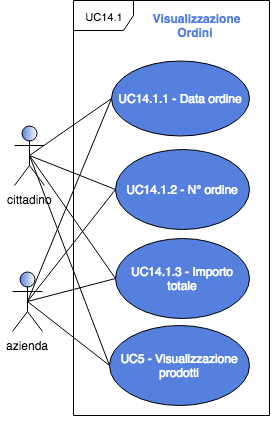
\includegraphics[width=5cm]{res/images/UC14-1VisualOrdini.png}
	\centering
	\caption{Visualizzazione degli ordini in modo dettagliato}
\end{figure}
\begin{itemize}
	\item \textbf{Attori Primari}: azienda, cittadino;
	\item \textbf{Descrizione}: alle aziende ed ai cittadini sono messe a disposizione diverse operazione per visualizzare e gestire gli ordini all'interno della piattaforma. In tale maniera vi è possibile avere un elenco dettagliato di tutti gli ordini;
	\item \textbf{Scenario principale}: l'utente visualizza e svolge alcune operazioni per gestiregli ordini;
	\item \textbf{Precondizione}: il sistema ha riconosciuto l'utente autenticato come azienda o cittadino e mette a disposizione tutte le pagine necessarie alla visualizzazione e gestione degli ordini;
	\item \textbf{Postcondizione}: l'utente ha visualizzato e/o gestito i propri ordini.
\end{itemize} 

\subsubsection{UC14.1.1 - Data ordine}
\begin{itemize}
	\item \textbf{Attori Primari}: azienda, cittadino;
	\item \textbf{Descrizione}: l'utente può visualizzare la data dell'ordine in questione;
	\item \textbf{Scenario principale}: l'utente visualizza la lista degli ordini;
	\item \textbf{Precondizione}: il sistema ha riconosciuto l'utente autenticato come azienda o cittadino e questo ha espresso la volontà di visualizzare la lista degli ordini per vedere le date degli stessi;
	\item \textbf{Postcondizione}: l'utente visualizza tale data.
\end{itemize}

\subsubsection{UC14.1.2 - N ordine}
\begin{itemize}
	\item \textbf{Attori Primari}: azienda, cittadino;
	\item \textbf{Descrizione}: l'utente può visualizzare il numero dell'ordine in questione;
	\item \textbf{Scenario principale}: l'utente visualizza la lista degli ordini;
	\item \textbf{Precondizione}: il sistema ha riconosciuto l'utente autenticato come azienda o cittadino e questo ha espresso la volontà di visualizzare la lista degli ordini per vedere i numeri degli stessi;
	\item \textbf{Postcondizione}: l'utente visualizza tale numero.
\end{itemize}

\subsubsection{UC14.1.3 - Importo netto}
\begin{itemize}
	\item \textbf{Attori Primari}: azienda, cittadino;
	\item \textbf{Descrizione}: l'utente può visualizzare l'importo netto dell'ordine in questione;
	\item \textbf{Scenario principale}: l'utente visualizza la lista degli ordini;
	\item \textbf{Precondizione}: il sistema ha riconosciuto l'utente autenticato come azienda o cittadino e questo ha espresso la volontà di visualizzare la lista degli ordini per vedere gli importi netti degli stessi;
	\item \textbf{Postcondizione}: l'utente visualizza tale importo.
\end{itemize}

\subsubsection{UC14.1.4 - Visualizzazione prodotti}
\begin{itemize}
	\item \textbf{Attori Primari}: azienda, cittadino;
	\item \textbf{Descrizione}: l'utente può visualizzare i prodotti inclusi nell'ordine in questione;
	\item \textbf{Scenario principale}: l'utente visualizza la lista degli ordini;
	\item \textbf{Precondizione}: il sistema ha riconosciuto l'utente autenticato come azienda o cittadino e questo ha espresso la volontà di visualizzare la lista degli ordini per vedere i prodotti inclusi negli stessi;
	\item \textbf{Postcondizione}: l'utente visualizza tali prodotti.
\end{itemize}

\subsubsection{UC14.1.5 - IVA}
\begin{itemize}
	\item \textbf{Attori Primari}: azienda, cittadino;
	\item \textbf{Descrizione}: l'utente può visualizzare l'importo dell'IVA dell'ordine in questione;
	\item \textbf{Scenario principale}: l'utente visualizza la lista degli ordini;
	\item \textbf{Precondizione}: il sistema ha riconosciuto l'utente autenticato come azienda o cittadino e questo ha espresso la volontà di visualizzare la lista degli ordini per vedere gli importi riguardanti l'IVA degli stessi;
	\item \textbf{Postcondizione}: l'utente visualizza tale importo.
\end{itemize}

\subsubsection{UC14.1.6 - Importo lordo}
\begin{itemize}
	\item \textbf{Attori Primari}: azienda, cittadino;
	\item \textbf{Descrizione}: l'utente può visualizzare l'importo lordo dell'ordine in questione;
	\item \textbf{Scenario principale}: l'utente visualizza la lista degli ordini;
	\item \textbf{Precondizione}: il sistema ha riconosciuto l'utente autenticato come azienda o cittadino e questo ha espresso la volontà di visualizzare la lista degli ordini per vedere gli importi lordi degli stessi;
	\item \textbf{Postcondizione}: l'utente visualizza tale importo.
\end{itemize}

\subsubsection{UC14.2 - Visualizzazione ordini in attesa di approvazione}
\begin{figure}[H]
	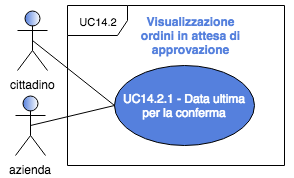
\includegraphics[width=5cm]{res/images/UC14-2.png}
	\centering
	\caption{Visualizzazione degli ordini in attesa di approazione}
\end{figure}
\begin{itemize}
	\item \textbf{Attori Primari}: azienda;
	\item \textbf{Descrizione}: all'azienda è messa a disposizione la possibilità di visualizzare e gestire gli ordini in attesa di approvazione, visualizzando la data ultima per la conferma;
	\item \textbf{Scenario principale}: l'utente visualizza gli ordini in attesa di approvazione;
		\item \textbf{Specializzazione}
	\begin{itemize}
		\item \textbf{UC14.4}: Visualizzazione degli ordini con modalità di pagamento immediato;
		\item \textbf{UC14.5}: Visualizzazione degli ordini con modalità di pagamento dilazionato.
	\end{itemize}
	\item \textbf{Precondizione}: il sistema ha riconosciuto l'utente autenticato come azienda e mette a disposizione tutte le pagine necessarie alla visualizzazione di questo tipo di ordini;
	\item \textbf{Postcondizione}: l'utente ha visualizzato e/o gestito i propri ordini in attesa di approvazione.
\end{itemize} 

\subsubsection{UC14.2.1 - Data ultima per la conferma}
\begin{itemize}
	\item \textbf{Attori Primari}: azienda;
	\item \textbf{Descrizione}: l'azienda può visualizzare la data ultima per la conferma dell'ordine in questione;
	\item \textbf{Scenario principale}: l'utente visualizza la lista degli ordini;
	\item \textbf{Precondizione}: il sistema ha riconosciuto l'utente autenticato come azienda e questo ha espresso la volontà di visualizzare la lista degli ordini per vedere le date di scadenza per l'ultima possibilità di esprimere la conferma;
	\item \textbf{Postcondizione}: l'utente visualizza tale data.
\end{itemize}

\subsubsection{UC14.3 - Visualizzazione Ordini con pagamento dilazionato}
\begin{figure}[H]
	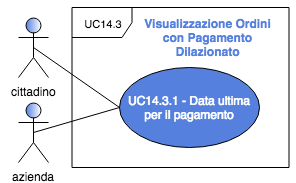
\includegraphics[width=5cm]{res/images/UC14-3.png}
	\centering
	\caption{Visualizzazione degli ordini con pagamento dilazionato}
\end{figure}
\begin{itemize}
	\item \textbf{Attori Primari}: azienda;
	\item \textbf{Descrizione}: alle aziende è messa a disposizione la possibilità di visualizzare e gestire gli ordini con pagamento dilazionato, visualizzando la data ultima per il pagamento;
	\item \textbf{Scenario principale}: l'utente visualizza gli ordini con modalità di pagamento dilazionato;
			\item \textbf{Specializzazione}
	\begin{itemize}
		\item \textbf{UC14.5}: Visualizzazione degli ordini con modalità di pagamento dilazionato;
		\item \textbf{UC14.6}: Visualizzazione delle vendite con modalità di pagamento dilazionato non concluse;
		\item \textbf{UC14.8}: Visualizzazione degli acquisti con modalità di pagamento dilazionato non concluse;
		\item \textbf{UC14.10}: Visualizzazione delle proposte d'acquisto in attesa di conferma.
	\end{itemize}
	\item \textbf{Precondizione}: il sistema ha riconosciuto l'utente autenticato come azienda e mette a disposizione tutte le pagine necessarie alla visualizzazione di questo tipo ordini;
	\item \textbf{Postcondizione}: l'utente ha visualizzato e/o gestito i propri acquisti con pagamento dilazionato.
\end{itemize} 

\subsubsection{UC14.3.1 - Data ultima per il pagamento}
\begin{itemize}
	\item \textbf{Attori Primari}: azienda;
	\item \textbf{Descrizione}: l'utente può visualizzare la data ultima per il pagamento dell'ordine in questione;
	\item \textbf{Scenario principale}: l'utente visualizza la lista degli ordini;
	\item \textbf{Precondizione}: il sistema ha riconosciuto l'utente autenticato come azienda e questo ha espresso la volontà di visualizzare la lista degli ordini per vedere le date di scadenza per l'ultima possibilità di effettuare il pagamento;
	\item \textbf{Postcondizione}: l'utente visualizza tale data.
\end{itemize}

\subsubsection{UC14.4 - Visualizzazione vendite con pagamento immediato}
\begin{itemize}
	\item \textbf{Attori Primari}: azienda;
	\item \textbf{Descrizione}: l'azienda può visualizzare la lista delle vendite la cui proposta d'ordine deve essere ancora accettata dall'azienda cliente, mostrando esclusivamente i risultati relativi alle vendite con modalità di pagamento immediato;
	\item \textbf{Scenario principale}: l'utente visualizza la lista delle vendite la cui proposta d'ordine deve essere ancora accettata dall'azienda cliente. Vengono mostrati esclusivamente i risultati relativi alle vendite con modalità di pagamento immediato;
	\item \textbf{Precondizione}: il sistema ha riconosciuto l'utente autenticato come azienda e questo ha espresso la volontà di visualizzare la lista delle vendite la cui proposta d'ordine deve ancora essere gestita dall'azienda cliente, visualizzando solo le vendite con modalità di pagamento immediato;
	\item \textbf{Postcondizione}: l'azienda visualizza tale lista.
\end{itemize}


\subsubsection{UC14.5 - Visualizzazione vendite con pagamento dilazionato}
\begin{itemize}
	\item \textbf{Attori Primari}: azienda;
	\item \textbf{Descrizione}: l'azienda può visualizzare la lista delle vendite la cui proposta d'ordine deve essere ancora accettata dall'azienda cliente, mostrando esclusivamente i risultati relativi alle vendite con modalità di pagamento dilazionato\glo;
	\item \textbf{Scenario principale}: l'utente visualizza la lista delle vendite la cui proposta d'ordine deve essere ancora accettata dall'azienda cliente. Vengono mostrati esclusivamente i risultati relativi alle vendite con modalità di pagamento dilazionato\glo;
	\item \textbf{Precondizione}: il sistema ha riconosciuto l'utente autenticato come azienda e questo ha espresso la volontà di visualizzare la lista delle vendite la cui proposta d'ordine deve ancora essere gestita dall'azienda cliente, visualizzando solo le vendite con modalità di pagamento dilazionato\glo;
	\item \textbf{Postcondizione}: l'azienda visualizza tale lista.
\end{itemize}


\subsubsection{UC14.6 - Visualizzazione vendite con pagamento dilazionato non concluse}
\begin{itemize}
	\item \textbf{Attori Primari}: azienda;
	\item \textbf{Descrizione}: l'azienda può visualizzare la lista delle vendite con pagamento dilazionato\glosp approvate, ma non ancora concluse, ovvero l'azienda-cliente deve ancora effettuare il pagamento;
	\item \textbf{Scenario principale}: l'utente visualizza la lista delle vendite con modalità di pagamento dilazionato\glosp accettate ma non ancora concluse;
	\item \textbf{Precondizione}: il sistema ha riconosciuto l'utente autenticato come azienda e questo ha espresso la volontà di visualizzare la lista delle vendite con modalità di pagamento dilazionato\glosp accettate ma non ancora concluse;
	\item \textbf{Postcondizione}: l'azienda visualizza tale lista.
\end{itemize}

\subsubsection{UC14 - Gestione ordini - parte acquisti}
\begin{figure}[h]
	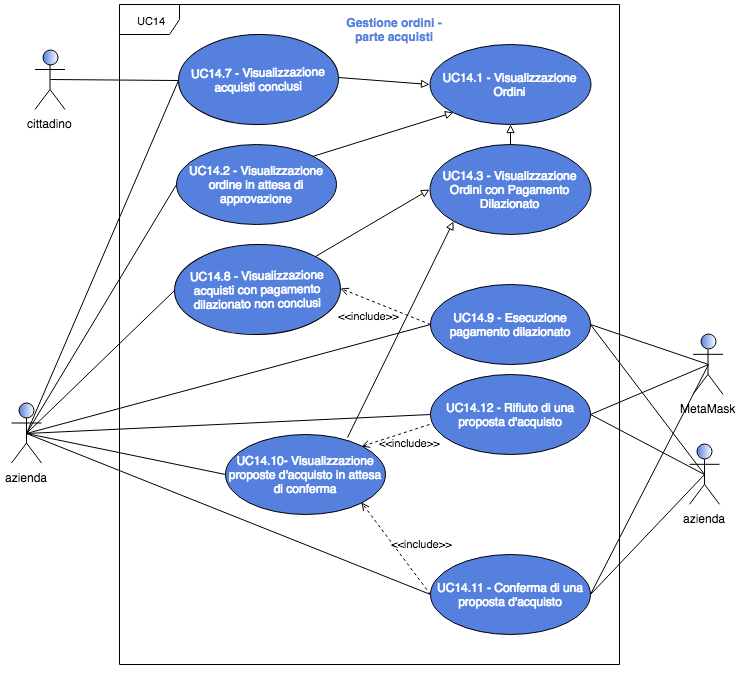
\includegraphics[width=10cm]{res/images/UC14ParteAcquisti.png}
	\centering
	\caption{Gestione degli ordini dal punto di vista delgli acquisti}
\end{figure}
\begin{itemize}
	\item \textbf{Attori Primari}: azienda, cittadino;
	\item \textbf{Descrizione}: alle aziende e ai cittadini sono messe a disposizione diverse operazione per visualizzare e gestire gli acquisti;
	\item \textbf{Scenario principale}: l'utente visualizza e svolge alcune operazioni per gestire gli ordini, queste includono:
	\begin{itemize}
		\item visualizzazione della data dell'ordine [UC14.1.1];
		\item visualizzazione del numero dell'ordine [UC14.1.2];
		\item visualizzazione dell'importo totale dell'ordine [UC14.1.3];
		\item visualizzazione dei prodotti inclusi nell'ordine [UC14.1.4].
	\end{itemize}
	Inoltre per gli ordini in attesa di approvazione è disponibile la data ultima per la conferma [UC14.2.1] e per quanto riguarda gli ordini con pagamento dilazionato,  la data ultima per il pagamento [UC14.3.1].
	\item \textbf{Specializzazione}
	\begin{itemize}
		\item \textbf{UC14.2}: Visualizzazione degli ordini in attesa di approvazione;
		\item \textbf{UC14.3}: Visualizzazione degli ordini con modalità di pagamento dilazionato;
		\item \textbf{UC14.7}: Visualizzazione degli acquisti conclusi.
	\end{itemize}
	\item \textbf{Precondizione}: il sistema ha riconosciuto l'utente autenticato come azienda o cittadino e mette a disposizione tutte le pagine necessarie alla visualizzazione e gestione degli acquisti.
	\item \textbf{Postcondizione}: l'utente ha visualizzato e/o gestito i propri ordini riguardanti gli acquisti.
\end{itemize} 
\subsubsection{UC14.7 - Visualizzazione acquisti conclusi}
\begin{itemize}
	\item \textbf{Attori Primari}: cittadino, azienda;
	\item \textbf{Descrizione}: l'utente può visualizzare la lista degli acquisti conclusi;
	\item \textbf{Scenario principale}: l'utente visualizza la lista degli acquisti conclusi;
	\item \textbf{Precondizione}: il sistema ha riconosciuto l'utente autenticato come azienda o cittadino e questo ha espresso la volontà di visualizzare la lista degli acquisti conclusi;
	\item \textbf{Postcondizione}: l'utente visualizza tale lista.
\end{itemize}
\subsubsection{UC14.8 - Visualizzazione acquisti con pagamento dilazionato non concluse}
\begin{itemize}
	\item \textbf{Attori Primari}: azienda;
	\item \textbf{Descrizione}: l'azienda può visualizzare la lista degli acquisti con pagamento dilazionato\glosp approvate, ma non ancora concluse, ovvero l'azienda-cliente deve ancora effettuare il pagamento;
	\item \textbf{Scenario principale}: l'utente visualizza la lista degli acquisti con modalità di pagamento dilazionato\glosp accettate ma non ancora concluse;
	\item \textbf{Precondizione}: il sistema ha riconosciuto l'utente autenticato come azienda e questo ha espresso la volontà di visualizzare la lista degli acquisti con modalità di pagamento dilazionato\glosp accettate ma non ancora concluse;
	\item \textbf{Postcondizione}: l'utente visualizza tale lista.
\end{itemize}
\subsubsection{UC14.9 - Esecuzione pagamento dilazionato}
\begin{itemize}
	\item \textbf{Attori Primari}: azienda-cliente;
	\item \textbf{Attori Secondaari}: azienda-venditrice, MetaMask\glo;
	\item \textbf{Descrizione}: l'azienda può effettuare il versamento della somma dovuta all'azienda-venditrice, relativa ad un pagamento dilazionato non ancora saldato. In questa maniera l'azienda-cliente può ricevere la fattura relativa a suddetto ordine;
	\item \textbf{Scenario principale}: l'utente visualizza la lista dei pagamenti dilazionati non ancora conclusi, preme sul tasto per il pagamento e segue la procedura attraverso MetaMask\glosp per effettuare il versamento;
	\item \textbf{Inclusione}: 
	\begin{itemize}
		\item \textbf{UC14.8}: l'utente che preme il pulsante per effettuare il pagamento deve obbligatoriamente aver richiesto la visualizzazione della lista dei pagamenti dilazionati non ancora conclusi;
	\end{itemize}
	\item \textbf{Precondizione}: il sistema ha riconosciuto l'utente autenticato come azienda e questo ha espresso la volontà effettuare il pagamento per saldare l'importo dovuto riguardante un pagamento dilazionato;
	\item \textbf{Postcondizione}: l'azienda-cliente ha effettuato il versamento della somma dovuta all'azienda-venditrice. L'azienda-cliente ha ricevuto la fattura per tale ordine è la può reperire nella sezione dedicata [UC16]. L'azienda-venditrice può ottenere le informazioni relative alla vendita nell'apposita sezione [UC14.5].
\end{itemize}
\subsubsection{UC14.10 - Visualizzazione proposte d'acquisto in attesa di conferma}
\begin{itemize}
	\item \textbf{Attori Primari}: azienda;
	\item \textbf{Descrizione}: l'azienda può visualizzare delle proposte d'acquisto che necessitano di conferma;
	\item \textbf{Scenario principale}: l'utente visualizza la lista delle proposte d'acquisto che necessitano di conferma. Per ognuna di esse ha a possibilità di confermare la proposta [UC14.11] o di rifiutarla [UC14.12];
	\item \textbf{Precondizione}: il sistema ha riconosciuto l'utente autenticato come azienda e questo ha espresso la volontà di visualizzare la lista delle proposte d'acquisto che necessitano di conferma;
	\item \textbf{Postcondizione}: l'azienda visualizza tale lista.
\end{itemize}
\subsubsection{UC14.11 - Conferma di una proposta di acquisto}
\begin{itemize}
	\item \textbf{Attori Primari}: azienda;
	\item \textbf{Descrizione}: l'azienda può confermare una proposta d'acquisto. Per confermare l'operazione verrà utilizzato MetaMask\glo;
	\item \textbf{Scenario principale}: l'utente visualizza una proposta d'acquisto che necessitano di conferma e decide di confermarla;
	\item \textbf{Inclusione}: 
	\begin{itemize}
		\item \textbf{UC14.10}: visualizzazione delle proposte d'acquisto in attesa di conferma.
	\end{itemize}
	\item \textbf{Precondizione}: il sistema ha riconosciuto l'utente autenticato come azienda ed ha mostrato la lista delle proposte d'acquisto che necessitano di conferma;
	\item \textbf{Postcondizione}: l'azienda ha confermato la proposta d'acquisto. La proposta non sarà più presente nella lista di attesa per la conferma, comparirà invece sulla lista degli acquisti conclusi [UC14.7]. L'acquisto comparirà come acquisto concluso, con esito positivo, nella lista delle vendite dell'azienda-venditrice [UC14.4, UC14.5]. Il sistema trasferisce l'ammontare trattenuto per l'ordine all'azienda-venditrice. L'azienda-cliente riceve nella pagina dedicata la fattura IVA relativa a questo ordine.
\end{itemize}
\subsubsection{UC14.12 - Rifiuto di una proposta di acquisto}
\begin{itemize}
	\item \textbf{Attori Primari}: azienda;
	\item \textbf{Descrizione}: l'azienda può rifiutare una proposta d'acquisto. Per confermare l'operazione verrà utilizzato MetaMask\glo;
	\item \textbf{Scenario principale}: l'utente visualizza una proposta d'acquisto che necessitano di conferma e decide di rifiutarla;
		\item \textbf{Inclusione}: 
	\begin{itemize}
		\item \textbf{UC14.10}: visualizzazione delle proposte d'acquisto in attesa di conferma.
	\end{itemize}
	\item \textbf{Precondizione}: il sistema ha riconosciuto l'utente autenticato come azienda ed ha mostrato la lista delle proposte d'acquisto che necessitano di conferma;
	\item \textbf{Postcondizione}: l'azienda ha rifiutato la proposta d'acquisto. La proposta non sarà più presente nella lista di attesa per la conferma. L'acquisto comparirà come acquisto concluso, con esito negativo, nella lista delle vendite dell'azienda-venditrice [UC14.4, UC14.5]. Il sistema ritorna l'ammontare trattenuto per l'ordine all'azienda-cliente.
\end{itemize}
